\begin{figure}[h!]
     \centering
    \captionsetup[sub]{font=small}
     \begin{minipage}[h!]{1\textwidth}
         \begin{subfigure}[b!]{0.3 \textwidth}
             \caption{}
             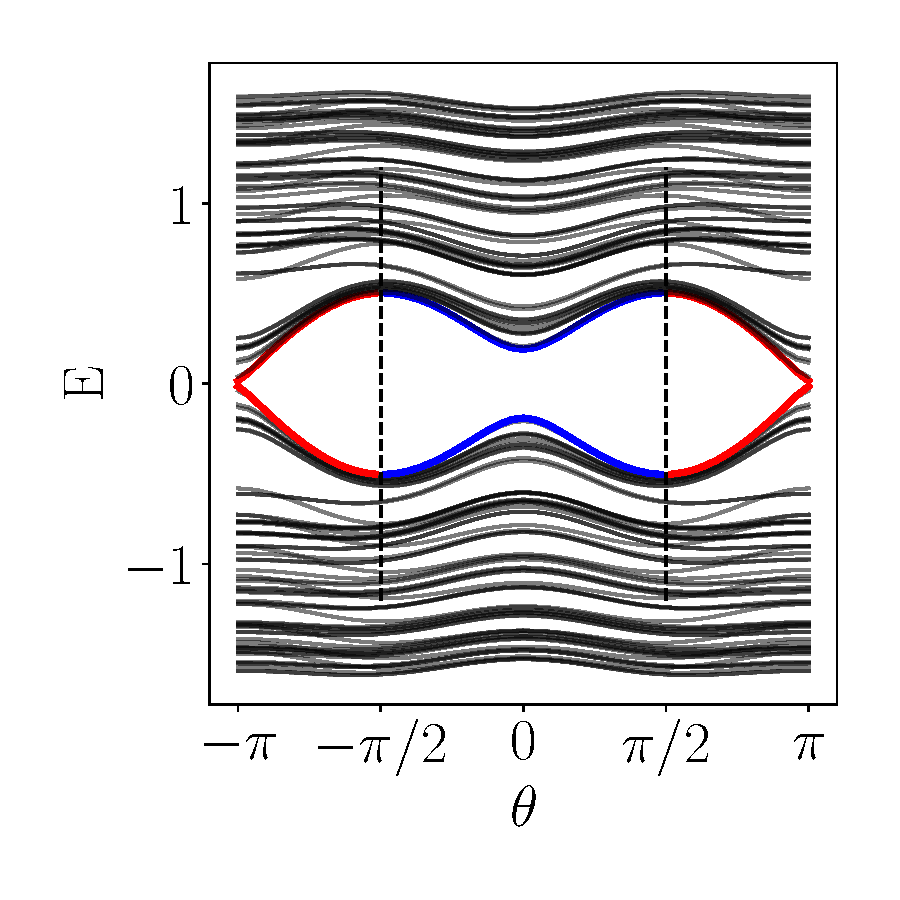
\includegraphics[width=\textwidth]{Imagenes/Resultados_pump_Fractal/x/param_pump_A=0.5x.pdf}
         \end{subfigure}\hspace*{-0.5em}
         \begin{subfigure}[b!]{0.35 \textwidth}
             \caption{}
             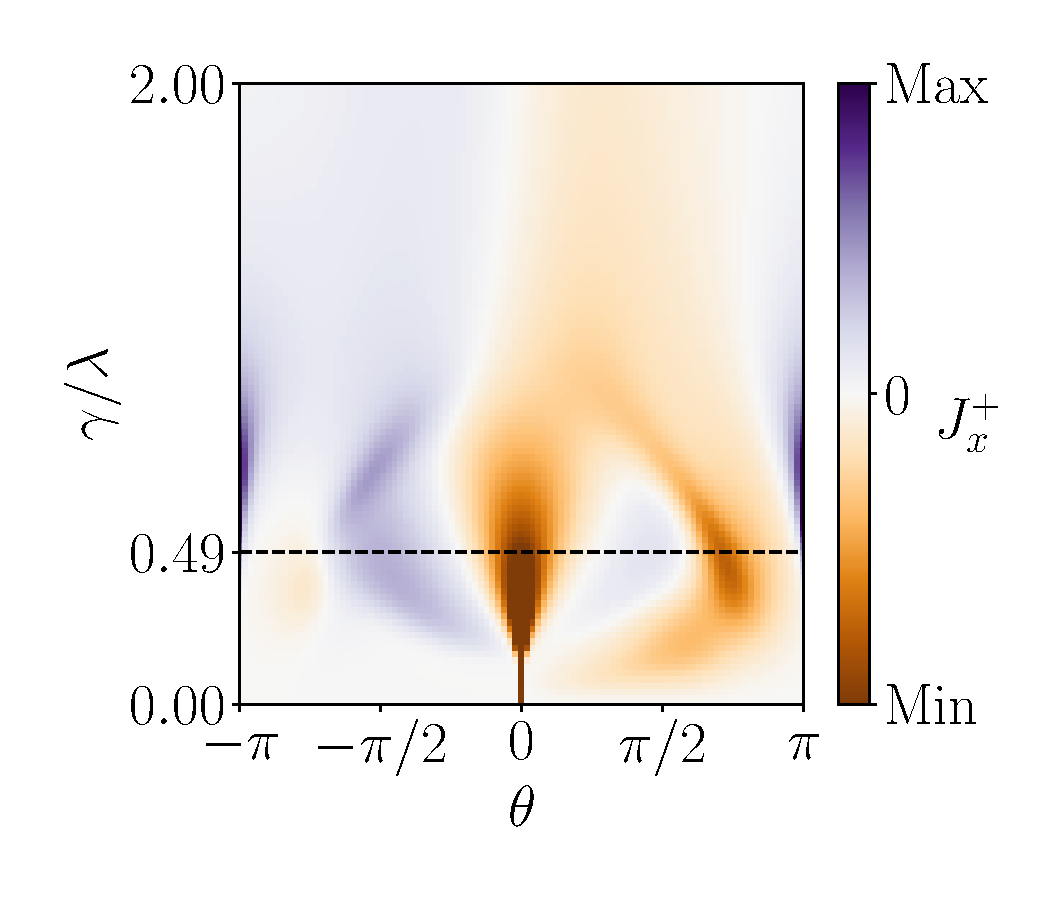
\includegraphics[width=\textwidth]{Imagenes/Resultados_pump_Fractal/x/current_square_pumpx.pdf}
         \end{subfigure}\hspace*{-0.5em}
         \begin{subfigure}[b!]{0.35 \textwidth}
             \caption{}
             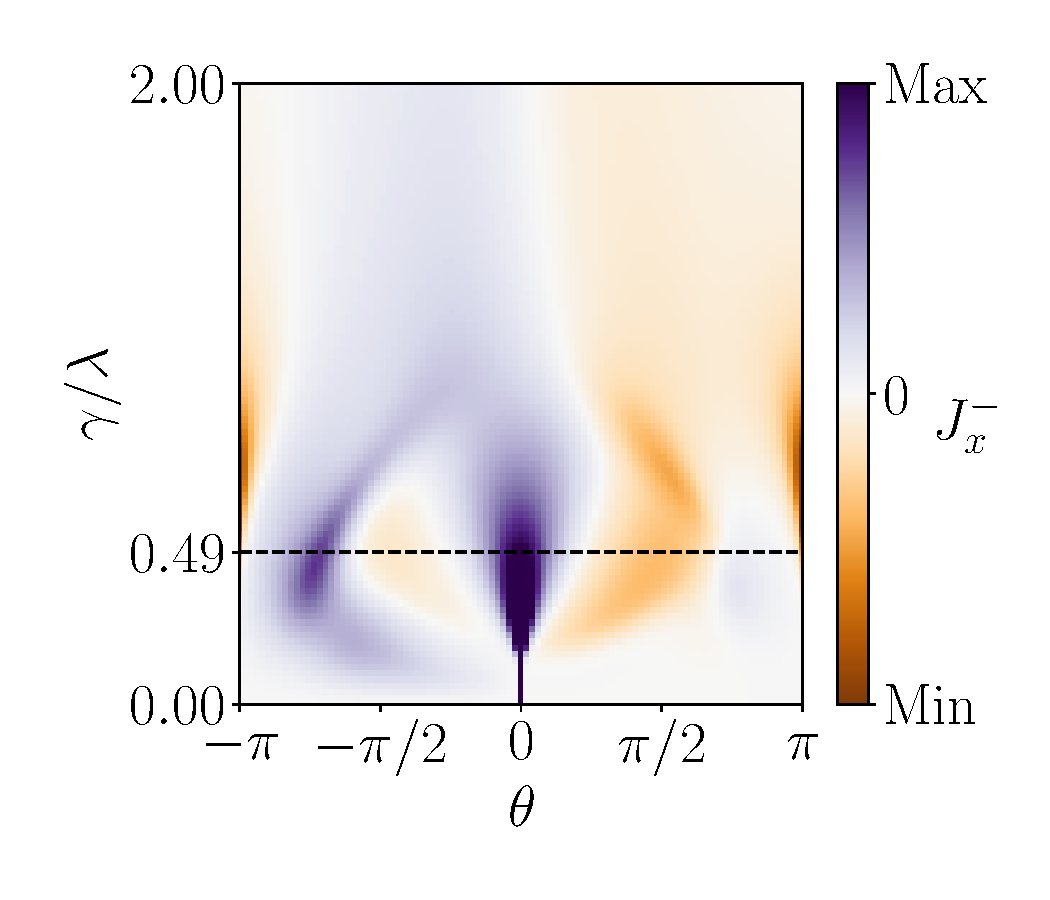
\includegraphics[width=\textwidth]{Imagenes/Resultados_pump_Fractal/x/current_square_pump_negx.pdf}
         \end{subfigure}\hspace*{-0.5em}
     \end{minipage}\vspace*{-1em}
     
     
     \begin{minipage}[h!]{1\textwidth}
         \begin{subfigure}[b!]{1.0 \textwidth}
             \caption{}
             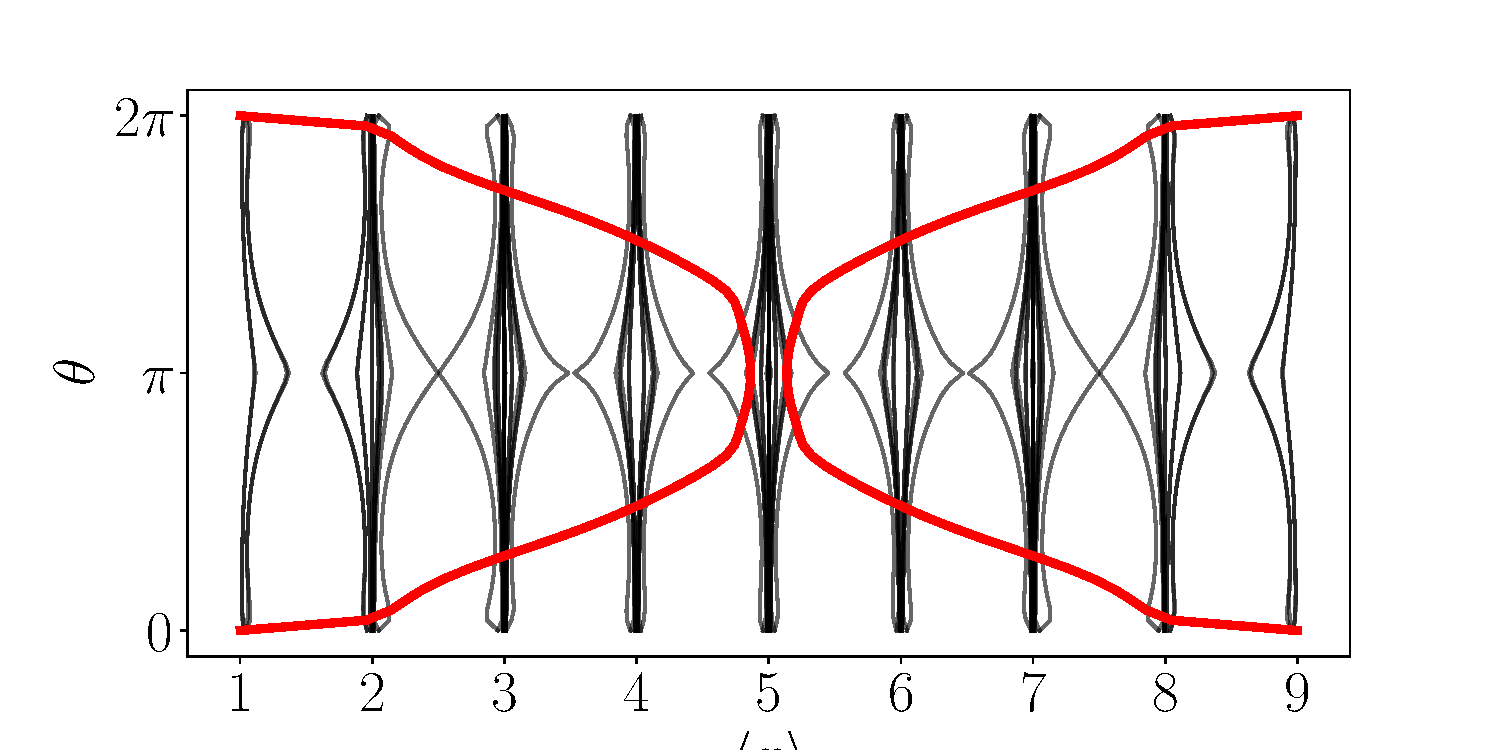
\includegraphics[width=\textwidth]{Imagenes/Resultados_pump_Fractal/x/wannier_centerx.pdf}
         \end{subfigure}\hspace*{-0.5em}
     \end{minipage}\vspace*{-1em}
     

     \begin{minipage}[h!]{1\textwidth}
        \begin{subfigure}[b!]{1.0 \textwidth}
            \caption{}
            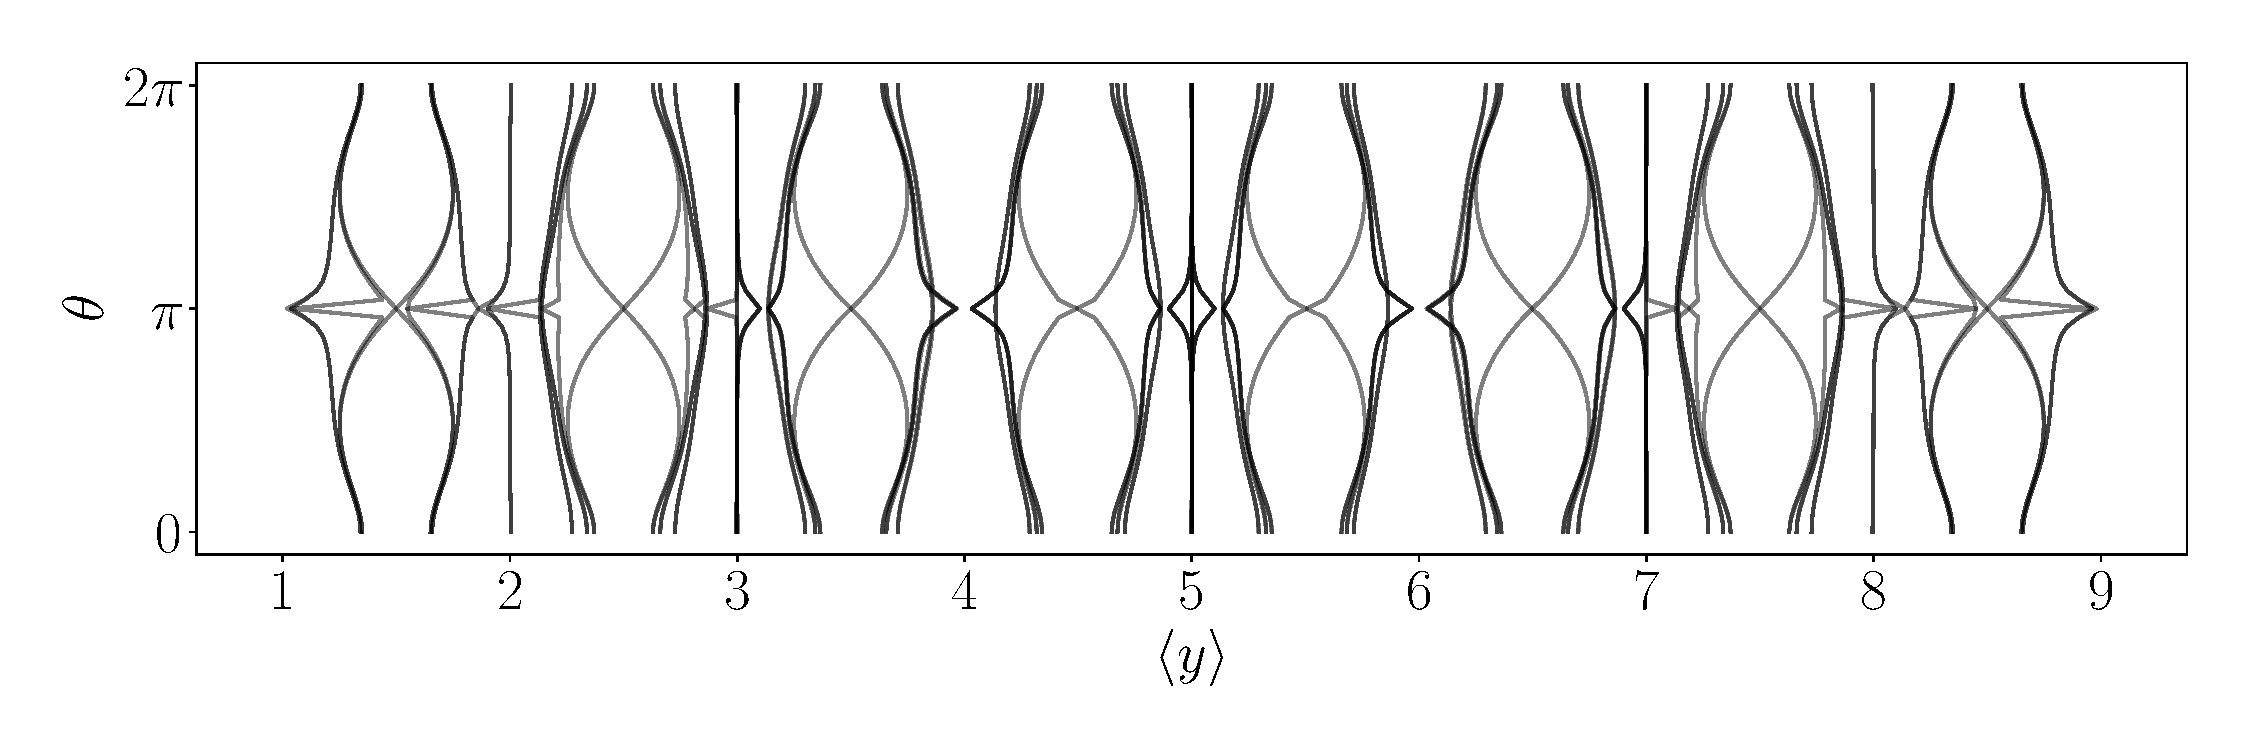
\includegraphics[width=\textwidth]{Imagenes/Resultados_pump_Fractal/x/wannier_centery.pdf}
        \end{subfigure}\hspace*{-0.5em}
    \end{minipage}\vspace*{-0.5em}
     
    \caption{\textbf{(a)} Variación del espectro de energías conforme cambia el parametro ciclico, las energias centrales corresponden a los estados de borde. En rojo se encuentra la fase topologica y en azul la fase trivial. \textbf{(b)-(c)} Flujo de densidad de corriente para diferentes elecciones de $\gamma$ y $\lambda$ conforme cambia el parametro $\theta$, para el espectro positivo y el espectro negativo de energias de borde, respectivamente. \textbf{(d)-(e)} Cambio de los centros de Wannier para el espectro de energias negativas, en \textbf{X} y \textbf{Y}. Estos resultados corresponden al modelo de bombeo BBH en una red de Sierpinski en la dirección \textbf{X}.}
    \label{fig:Pump_fractal_x}
\end{figure}